\section{Multizone Interface Connectivity}
\label{s:connectivity}
\thispagestyle{plain}

This section defines structures for describing multizone interface
connectivity for 1-to-1 abutting, mismatched abutting, and overset
type interfaces.  The different types of zone interfaces are
described in \autoref{s:interface_types}.  All interface connectivity
information pertaining to a given zone is grouped together in a
|ZoneGridConnectivity_t| structure entity; this in turn is contained
in a zone structure entity (see the definition of |Zone_t| in
\autoref{s:Zone}).

Before presentation of the structure definitions, a few design features
require comment.
All indices used to describe interfaces are the dimensionality
(\fort{IndexDimension}) of the grid, even when they are used to describe
lower-dimensional zonal boundaries for abutting interfaces.
The alternative for structured zones that was not chosen is to use
lower-dimensional indices for lower-dimensional interfaces (e.g., for a
3-D grid, use two-dimensional indices for describing grid planes that
are interfaces).
Both alternatives offer trade-offs.
The lower-dimensional indices require cyclic notation conventions and
additional identification of face location; whereas, full-dimensional
indices result in one redundant index component when describing points
along a grid plane.
We decided that full-dimensional indices would be more usable and less
error prone in actual implementation.

A major consequence of this decision is that connectivity information
for describing mismatched abutting interfaces and overset interfaces
can be merged into a single structure, \fort{GridConnectivity\_t} (see
\autoref{s:GridConnectivity} below).
In fact, this single structure type can be used to describe all zonal
interfaces.

A second design choice was to duplicate all 1-to-1 abutting interface
information within the CGNS database.  It is possible to describe
a given 1-to-1 interface with a single set of connectivity data.
In contrast, mismatched and overset interfaces require different
connectivity information when the roles of receiver and donor zones
are interchanged.  Therefore, a given mismatched or overset interface
requires two sets of connectivity data within the database.  The
decision to force two sets of connectivity data (one contained in each
of the |Zone_t| entities for the two adjacent zones) for each 1-to-1
interface makes the connectivity structures for all interface types
look and function similarly.  It also fits better with the zone-by-zone
hierarchy chosen for the CGNS database.  The minor penalty in data
duplication was deemed worth the advantages gained.

Note that it is a CGNS design intent that a given zone boundary segment
or location should at most be defined (or covered) by either a boundary
condition or a multizone interface connectivity, but not by both.

\subsection{Zonal Connectivity Structure Definition: \texttt{ZoneGridConnectivity\_t}} 
\label{s:ZoneGridConnectivity}

All multizone interface grid connectivity information pertaining to
a given zone is contained in the |ZoneGridConnectivity_t| structure.
This includes abutting interfaces (1-to-1 and general mismatched),
overset-grid interfaces, and overset-grid holes.

\begin{alltt}
  ZoneGridConnectivity\_t< int IndexDimension, int CellDimension > :=
    \{
    List( Descriptor\_t Descriptor1 ... DescriptorN ) ;                      (o)

    List( GridConnectivity1to1\_t<IndexDimension>
          GridConnectivity1to11 ... GridConnectivity1to1N ) ;               (o)

    List( GridConnectivity\_t<IndexDimension, CellDimension>
          GridConnectivity1 ... GridConnectivityN ) ;                       (o)

    List( OversetHoles\_t<IndexDimension> 
          OversetHoles1 ... OversetHolesN ) ;                               (o)

    List( UserDefinedData\_t UserDefinedData1 ... UserDefinedDataN ) ;       (o)
    \} ;
\end{alltt}

\begin{notes}
\item
 Default names for the \fort{Descriptor\_t}, \fort{GridConnectivity1to1\_t},
 \fort{GridConnectivity\_t}, \fort{OversetHoles\_t}, and
 \fort{UserDefinedData\_t}
 lists are as shown; users may choose other legitimate names.
 Legitimate names must be unique 
 within a given instance of |ZoneGridConnectivity_t|.
\item
 All lists within the |ZoneGridConnectivity_t| structure may be empty.
\end{notes}

|ZoneGridConnectivity_t| requires two structure parameters,
|IndexDimension|, which is passed onto all connectivity substructures, and
\fort{CellDimension}, which is passed to \fort{GridConnectivity\_t} only.

Connectivity information for 1-to-1 or matched multizone interfaces is
contained in the \texttt{GridConnectivity1to1\_t} structure.
Abutting and overset connectivity is contained in the
\texttt{GridConnectivity\_t} structure, and overset-grid holes are
identified in the \texttt{OversetHoles\_t} structure.

The \fort{UserDefinedData\_t} data structure allows arbitrary
user-defined data to be stored in \fort{Descriptor\_t} and
\fort{DataArray\_t} children without the restrictions or implicit
meanings imposed on these node types at other node locations.

\subsection{1-to-1 Interface Connectivity Structure Definition: \texttt{GridConnectivity1to1\_t}}
\label{s:GridConnectivity1to1}

\fort{GridConnectivity1to1\_t} only applies to structured zones
interfacing with structured donors and whose interface is a logically
rectangular region.
It contains connectivity information for a multizone interface patch
that is abutting with 1-to-1 matching between adjacent zone indices
(also referred to as C0 connectivity).
An interface patch is the subrange of the face of a zone that touches
one and only one other zone.
This structure identifies the subrange of indices for the two adjacent
zones that make up the interface and gives an index transformation from
one zone to the other.
It also identifies the name of the adjacent zone.

All the interface patches for a given zone are contained in the
|ZoneGridConnectivity_t| entity for that zone.
If a face of a zone touches several other zones (say $N$), then $N$
different instances of the |GridConnectivity1to1_t| structure must be
included in the zone to describe each separate interface patch.
This convention requires that a single interface patch be described
twice in the database---once for each adjacent zone.

\begin{alltt}
  GridConnectivity1to1\_t< int IndexDimension > :=
    \{
    List( Descriptor\_t Descriptor1 ... DescriptorN ) ;                      (o)

    int[IndexDimension] Transform ;                                         (o/d)

    IndexRange\_t<IndexDimension> PointRange ;                               (r)
    IndexRange\_t<IndexDimension> PointRangeDonor ;                          (r)

    Identifier(Zone\_t) ZoneDonorName ;                                      (r)

    GridConnectivityProperty\_t GridConnectivityProperty ;                   (o)

    List( UserDefinedData\_t UserDefinedData1 ... UserDefinedDataN ) ;       (o)

    int Ordinal ;                                                           (o)
    \} ;
\end{alltt}

\begin{notes}
\item Default names for the \fort{Descriptor\_t} and
      \fort{UserDefinedData\_t} lists are as shown; users may choose
      other legitimate names.
      Legitimate names must be unique within a given instance of
      \fort{GridConnectivity1to1\_t} and shall not include the
      names \fort{GridConnectivityProperty}, \fort{PointRange},
      \fort{PointRangeDonor}, \fort{Transform}, or \fort{Ordinal}.
\item If \fort{Transform} is absent, then its default value is
      $[+1,+2,+3]$.
\item \fort{ZoneDonorName} must be equated to a zone identifier
      within the current CGNS database (i.e., it must be equal to
      one of the \fort{Zone\_t} identifiers contained in the current
      \fort{CGNSBase\_t} entity).
\item Beginning indices of \fort{PointRange} and \fort{PointRangeDonor}
      must coincide (i.e., must be the same physical point); ending
      indices of \fort{PointRange} and \fort{PointRangeDonor} must also
      coincide.
\item Elements of \fort{Transform} must be signed integers in the range
      \texttt{-IndexDimension}, $\ldots$,
      \texttt{+IndexDimension}; element magnitudes may not be
      repeated.
      In 3-D allowed elements are $0$, $\pm1$, $\pm2$, $\pm3$.
\end{notes}

\fort{PointRange} contains the subrange of indices that makes up the
interface patch in the current zone (i.e., that \fort{Zone\_t} entity
that contains the given instance of \fort{GridConnectivity1to1\_t}).
\fort{PointRangeDonor} contains the interface patch subrange of indices
for the adjacent zone (whose identifier is given by \fort{ZoneDonorName}).
By convention the indices contained in \fort{PointRange} and
\fort{PointRangeDonor} refer to vertices.

|Transform| contains a short-hand notation for the transformation matrix
describing the relation between indices of the two adjacent zones.
The transformation matrix itself has rank |IndexDimension| and contains
elements $+1$, $-1$ and $0$; it is orthonormal and its inverse is its
transpose.
The transformation matrix (|T|) works as follows: if |Index1| and
|Index2| are the indices of a given point on the interface, where
|Index1| is in the current zone and |Index2| is in the adjacent zone,
then their relationship is,
\begin{alltt}
  Index2 = T.(Index1 - Begin1) + Begin2 

  Index1 = Transpose[T].(Index2 - Begin2) + Begin1 
\end{alltt}
where the ``\texttt{.}'' notation indicates matrix-vector multiply.
\texttt{Begin1} and \texttt{End1} are the subrange indices contained
in \texttt{PointRange}, and \texttt{Begin2} and \texttt{End2} are the
subrange indices contained in \texttt{PointRangeDonor}.

The short-hand notation used in |Transform| is as follows: each element
shows the image in the adjacent zone's face of a positive index increment in
the current zone's face.  The first element is the image of a positive
increment in $i$; the second element is the image of an increment in $j$; and
the third (in 3-D) is the image of an increment in $k$ on the
current zone's face.  For 3-D, the transformation matrix |T| is constructed
from |Transform = [|$\pm a$, $\pm b$, $\pm c$|]| as follows:
\def\abs#1{{\rm abs}( #1 )}
\def\del#1{{\rm del}( #1 )}
\def\sgn#1{{\rm sgn}( #1 )}
$$
|T| = \left[
\begin{array}{ccc}
 \sgn{a} \, \del{a - 1} & \sgn{b} \, \del{b - 1} & \sgn{c} \, \del{c - 1} \\
 \sgn{a} \, \del{a - 2} & \sgn{b} \, \del{b - 2} & \sgn{c} \, \del{c - 2} \\
 \sgn{a} \, \del{a - 3} & \sgn{b} \, \del{b - 3} & \sgn{c} \, \del{c - 3} 
\end{array} \right],
$$
where,
$$
\sgn{x} \equiv \cases{ +1, &if $x \ge 0$ \cr -1, & if $x < 0$} 
 \quad\quad
\del{x - y} \equiv \cases{ 1, &if $\abs{x} = \abs{y}$ \cr 0, & otherwise}
$$
For example, |Transform = [|$-2$, $+3$, $+1$|]| gives the transformation
matrix,
$$
|T| = \left[
\begin{array}{rrr}
  0 &  0 & +1 \\
 -1 &  0 &  0 \\
  0 & +1 &  0 
\end{array} \right].
$$

For establishing relationships between adjacent and current zone indices
lying on the interface itself, one of the elements of |Transform| is
superfluous since one component of both interface indices remains constant.
It is therefore acceptable to set that element of |Transform| to zero.

If the transformation matrix is used for continuation of computational
coordinates into the adjacent zone (e.g., to find the location of a rind point
in the adjacent zone), then all elements of |Transform| are needed.  If the
above mentioned superfluous element is set to zero, it can be easily
regenerated from |PointRange| and |PointRangeDonor| and the grid sizes of the
two zones.  This is done by determining the faces represented by |PointRange|
and |PointRangeDonor| (i.e., $i$-min, $i$-max, $j$-min, etc.).  If one is a
minimum face and the other a maximum face, then the sign of the missing
element in |Transform| is ``$+$'', and the value of the missing element in the
transformation matrix (|T|) is $+1$.  If the faces are both minimums or are
both maximums, the sign is ``$-$''.  Next, the position and magnitude of the
element in |Transform|, and hence the row and column in the transformation
matrix, is given by the combinations of $i$, $j$ and $k$ faces for the two.
For example, if |PointRange| represents a $j$-min or $j$-max face and
|PointRangeDonor| represents an $i$-min or $i$-max face, then the missing
element's position in |Transform| is 2 and its magnitude is 1 (i.e.,
|Transform = [|$*$, $\pm 1$, $*$|]|).

Note also that the transform matrix and the two index pairs overspecify the
interface patch.  For example, |End2| can be obtained from |Transform|,
|Begin1|, |End1| and |Begin2|.

A \fort{GridConnectivityProperty\_t} data structure, described in
\autoref{s:GridConnectivityProperty}, may be used to record special
properties associated with particular connectivity patches, such as a
periodic interface, or an interface where data is to be averaged in some
way.

The \fort{UserDefinedData\_t} data structure allows arbitrary
user-defined data to be stored in \fort{Descriptor\_t} and
\fort{DataArray\_t} children without the restrictions or implicit
meanings imposed on these node types at other node locations.

|Ordinal| is user-defined and has no restrictions on the values that it can
contain.  It is included for backward compatibility to assist implementation
of the CGNS system into applications whose I/O depends heavily on the
numbering of zone interfaces.  Since there are no restrictions on the values
contained in |Ordinal| (or that |Ordinal| is even provided), there is no
guarantee that the interfaces in an existing CGNS database
will have sequential values from 1 to $N$ without holes or repetitions.  Use
of |Ordinal| is discouraged and is on a user-beware basis.

\subsection{1-to-1 Interface Connectivity Examples}
\label{s:cnct_1to1_example}

This section contains two examples of structure entities for describing
the connectivity for struc\-tured-zone 1-to-1 abutting multizone
interfaces.
\hyperref[s:twozone]{Appendix~\ref*{s:twozone}} contains additional
examples of 1-to-1 interfaces.

\begin{example}{1-to-1 Abutting of Complete Faces}
\label{ex:struct_1to1}

Two zones have the same orientation; zone 1 is $9\cross 17\cross 11$ and 
zone 2 is $9\cross 17\cross 21$.
The $k$-max face of zone 1 abuts the $k$-min face of zone 2.
Contained in the structure entities of zone 1 is the following interface
structure:
\begin{alltt}
  GridConnectivity1to1\_t<3> Zone1/ZoneGridConnectivity/KMax =
    \{\{
    int[3] Transform = [1,2,3] ;
    IndexRange\_t<3> PointRange =
      \{\{
      int[3] Begin = [1,1,11] ;
      int[3] End   = [9,17,11] ;
      \}\} ;
    IndexRange\_t<3> PointRangeDonor =
      \{\{
      int[3] Begin = [1,1,1] ; 
      int[3] End   = [9,17,1] ;
      \}\} ;
    Identifier(Zone\_t) ZoneDonorName = Zone2 ;
    \}\} ;
\end{alltt}
Contained in the structure entities of zone 2 is the following:
\begin{alltt}
  GridConnectivity1to1\_t<3> Zone2/ZoneGridConnectivity/KMin =
    \{\{
    int[3] Transform = [1,2,3] ;
    IndexRange\_t<3> PointRange =
      \{\{
      int[3] Begin = [1,1,1] ; 
      int[3] End   = [9,17,1] ;
      \}\} ;
    IndexRange\_t<3> PointRangeDonor =
      \{\{
      int[3] Begin = [1,1,11] ;
      int[3] End   = [9,17,11] ;
      \}\} ;
    Identifier(Zone\_t) ZoneDonorName = Zone1 ;
    \}\} ;
\end{alltt}
\end{example}
This example assumes zones 1 and 2 have the identifiers |Zone1| and |Zone2|,
respectively.    

\begin{example}{1-to-1 Abutting, Complete Face to a Subset of a Face}
\label{ex:1to1b}

\begin{figure}[!htb]
   \centering
   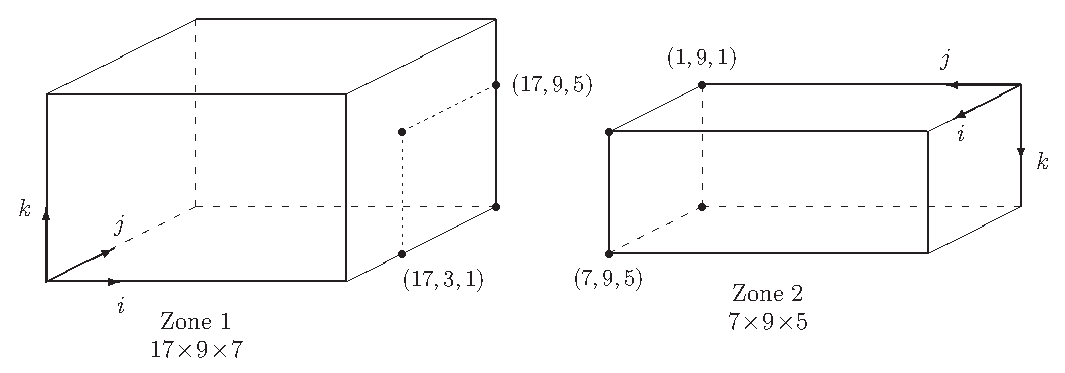
\includegraphics[width=\textwidth]{cnct.figs/cnct_1to1}
   \caption{Example Interface for 1-to-1 Connectivity}
   \label{f:cnct_1to1}
\end{figure}

\autoref{f:cnct_1to1} shows a more complex 1-to-1 abutting interface, where
the entire $j$-max face of zone 2 coincides with a subset of the $i$-max
face of zone 1.
This situation would result in the following connectivity structures:
\begin{alltt}
  GridConnectivity1to1\_t<3> Zone1/ZoneGridConnectivity/IMax =
    \{\{
    int[3] Transform = [-2,-1,-3] ;
    IndexRange\_t<3> PointRange =
      \{\{
      int[3] Begin = [17,3,1] ;
      int[3] End   = [17,9,5] ;
      \}\} ;
    IndexRange\_t<3> PointRangeDonor =
      \{\{
      int[3] Begin = [7,9,5] ; 
      int[3] End   = [1,9,1] ;
      \}\} ;
    Identifier(Zone\_t) ZoneDonorName = Zone2 ;
    \}\} ;
\end{alltt}

\begin{alltt}
  GridConnectivity1to1\_t<3> Zone2/ZoneGridConnectivity/JMax =
    \{\{
    int[3] Transform = [-2,-1,-3] ;
    IndexRange\_t<3> PointRange =
      \{\{
      int[3] Begin = [1,9,1] ;
      int[3] End   = [7,9,5] ;
      \}\} ;
    IndexRange\_t<3> PointRangeDonor =
      \{\{
      int[3] Begin = [17,9,5] ; 
      int[3] End   = [17,3,1] ;
      \}\} ;
    Identifier(Zone\_t) ZoneDonorName = Zone1 ;
    \}\} ;
\end{alltt}
\end{example}
This example also assumes zones 1 and 2 have the identifiers |Zone1| and
|Zone2|, respectively.
Note that the index transformation matrix for both this and the previous
examples is symmetric; hence, the value of |Transform| is identical for
both members of the interface pair.
In general this will not always be the case.

\subsection{General Interface Connectivity Structure Definition: \texttt{GridConnectivity\_t}}
\label{s:GridConnectivity}

|GridConnectivity_t| contains connectivity information for generalized
multizone interfaces, and may be used for any mix of structured and
unstructured zones.
Its purpose is to describe mismatched-abutting and overset interfaces,
but can also be used for 1-to-1 abutting interfaces.

For abutting interfaces that are not 1-to-1, also referred to as patched
or mismatched, an interface patch is the subrange of the face of a zone
that touches one and only one other zone.
This structure identifies the subrange of indices (or array of indices)
that make up the interface and gives their image in the adjacent (donor)
zone.
It also identifies the name of the adjacent zone.
If a given face of a zone touches several (say $N$) adjacent zones,
then $N$ different instances of |GridConnectivity_t| are needed to
describe all the interfaces.
For a single abutting interface, two instances of |GridConnectivity_t|
are needed in the database -- one for each adjacent zone.

For overset interfaces, this structure identifies the fringe points of
a given zone that lie in one and only one other zone.  If the fringe
points of a zone lie in several (say $N$) overlapping zones, then $N$
different instances of |GridConnectivity_t| are needed to describe the
overlaps.  It is possible with overset grids that a single fringe point
may actually lie in several overlapping zones (though in typical usage,
linkage to only one of the overlapping zones is kept).  There is no
restriction against a given fringe point being contained within multiple
instances of |GridConnectivity_t|; therefore, this structure allows the
description of a single fringe point lying in several overlapping zones.

\begin{alltt}
  GridConnectivityType\_t := Enumeration(
    GridConnectivityTypeNull,
    GridConnectivityTypeUserDefined,
    Overset,
    Abutting,
    Abutting1to1 ) ;

  GridConnectivity\_t< int IndexDimension, int CellDimension > :=
    \{
    List( Descriptor\_t Descriptor1 ... DescriptorN ) ;                      (o)

    GridConnectivityType\_t GridConnectivityType ;                           (o/d)

    GridLocation\_t GridLocation ;                                           (o/d)

    IndexRange\_t<IndexDimension> PointRange ;                               (o:r)
    IndexArray\_t<IndexDimension, PointListSize, int>  PointList ;           (r:o)
    IndexArray\_t<IndexDimension, PointListSize, int>  PointListDonor ;      (o)
    IndexArray\_t<IndexDimension, PointListSize, int>  CellListDonor ;       (o)

    Identifier(Zone\_t) ZoneDonorName ;                                      (r)

    DataArray\_t <real, 2, [CellDimension, PointListSize]> InterpolantsDonor (o)

    GridConnectivityProperty\_t GridConnectivityProperty ;                   (o)

    List( UserDefinedData\_t UserDefinedData1 ... UserDefinedDataN ) ;       (o)

    int Ordinal ;                                                           (o)
    \} ;
\end{alltt}

\begin{notes}
\item Default names for the \texttt{Descriptor\_t} and
      \texttt{UserDefinedData\_t} lists are as shown; users may choose
      other legitimate names.
      Legitimate names must be unique within a given instance of
      \texttt{GridConnectivity\_t} and shall not include the names
      \texttt{CellListDonor}, \texttt{GridConnectivityProperty},
      \texttt{GridConnectivityType}, \texttt{GridLocation},
      \texttt{InterpolantsDonor}, \texttt{Ordinal}, \texttt{PointList},
      \texttt{PointListDonor}, or \texttt{PointRange}.
\item \texttt{ZoneDonorName} must be equated to a zone identifier
      within the current CGNS database (i.e., it must be equal to one
      of the \texttt{Zone\_t} identifiers contained in the current
      \texttt{CGNSBase\_t} entity).
\item If \texttt{GridConnectivityType} is absent, then its default value
      is \texttt{Overset}.
\item For \texttt{Abutting} or \texttt{Abutting1to1} interfaces,
      \texttt{GridLocation} can be either \texttt{Vertex} or
      \texttt{FaceCenter}.
      When \texttt{GridLocation} is set to \texttt{Vertex}, then
      \texttt{PointList} or \texttt{PointRange} refer to node indices,
      for both structured and unstructured grids.
      When \texttt{GridLocation} is set to \texttt{FaceCenter}, then
      \texttt{PointList} or \texttt{PointRange} refer to face elements.
      Face elements are indexed using different methods depending if the
      zone is structured or unstructured.
      For a structured zone, face elements are indexed using the
      minimum of the connecting vertex indices, as described in
      \autoref{s:structgrid}.
      For an unstructured zone, face elements are indexed using their
      element numbering, as defined in the \texttt{Elements\_t} data
      structures.
      For \texttt{Overset} interfaces, \texttt{GridLocation} can be
      either \texttt{Vertex} or \texttt{CellCenter}, allowing the
      description of the overlap region in the receiver zone to be
      consistent with the grid location used for storing the flow
      solution.
      If \texttt{GridLocation} is absent, then its default value is
      \texttt{Vertex}.
\item One of \texttt{PointRange} and \texttt{PointList} must be
      specified, but not both.
\item If \texttt{PointRange} is specified, then an index ordering
      convention is needed to map receiver-zone grid points to
      donor-zone grid points.
      FORTRAN multidimensional array ordering is used.
\item If \texttt{GridConnectivityType} is \texttt{Abutting1to1} or
      \texttt{Abutting}, then \texttt{PointRange} or \texttt{PointList}
      must define points associated with a face subrange (if
      the zone is structured, all points must be in a single
      computational grid plane); the donor-zone grid locations defined
      by \texttt{PointListDonor} or \texttt{CellListDonor} must also be
      associated with a face subrange.
\item If donor information is given, either \texttt{PointListDonor}
      alone, or \texttt{CellListDonor} with or without
      \texttt{InterpolantsDonor}, must be used.
      The use of \texttt{PointListDonor} is restricted to
      \texttt{Abutting1to1}, whereas \texttt{CellListDonor} can be used
      for any interface type.
\item Thus, for a \texttt{GridConnectivityType} that is not
      \texttt{Abutting1to1}, there are three allowable levels of
      description concerning the connectivity information: (a) full,
      giving \texttt{ZoneDonorName} with \texttt{CellListDonor}
      plus \texttt{InterpolantsDonor}; (b) partial, giving
      \texttt{ZoneDonorName} with \texttt{CellListDonor} but
      no \texttt{InterpolantsDonor}; or (c) minimal, giving
      \texttt{ZoneDonorName} only.
\end{notes}

The type of multizone interface connectivity may be \fort{Overset},
\fort{Abutting}, or \fort{Abutting1to1}.
\fort{Overset} refers to zones that overlap; for a 3-D configuration the
overlap is a 3-D region.
|Abutting| refers to zones that abut or touch, but do not overlap (other
than the vertices and faces that make up the interface).
|Abutting1to1| is a special case of abutting interfaces where grid lines
are continuous across the interface and all vertices on the interface
are shared by the two adjacent zones.
See \autoref{s:interface_types} for a description of the three different
types of interfaces.

The interface grid points within the receiver zone may be specified by
|PointRange| if they constitute a logically rectangular region (e.g., an
abutting interface where an entire face of the receiver zone abuts with a
part of a face of the donor zone).  In all other cases, |PointList| should be
used to list the receiver-zone grid points making up the interface.
For a structured-to-structured interface, all indices in |PointRange| or
|PointList| should have one index element in common (see note 7).

\texttt{GridLocation} identifies the location of indices within the
receiver zone described by \texttt{PointRange} or \texttt{PointList}.
It also identifies the location of indices defined by
\texttt{PointListDonor} in the donor zone.
\texttt{GridLocation} does \emph{not} apply to \texttt{CellListDonor} or 
\texttt{InterpolantsDonor}.
The \texttt{CellListDonor} is always an index or indices that define a
particular cell or element, while the \texttt{InterpolantsDonor} defines
an interpolation value relative to the cell/element \emph{vertices}.
In other words, when using \texttt{InterpolantsDonor}, the interpolants
are always given with respect to the vertices of the donor zone.
\texttt{InterpolantsDonor} is currently only defined for structured
grids and certain basic unstructured grid element types.

For structured grids, the interpolant value is given along each index
direction, depending on the location within the cell.
For example, if the point is located within the cell at a position 75\%
in the $i$-direction, 41\% in the $j$-direction, and 20\% in the
$k$-direction, then \texttt{InterpolantsDonor} values ($r$, $s$, $t$)
would be (0.75, 0.41, 0.20).

The interpolation function is a linear combination of the $x$, $y$, and
$z$ values at the surrounding nodes:
$$
d = \sum_{i=1}^{N} W_i \cdot d_i
$$
where $d$ is the $x$, $y$, or $z$ value at an interior point in the
cell, $d_i$ is the $x$, $y$, or $z$ value at node $i$, and $W_i$ is a
weight at node $i$.
The weights are functions of the parametric variables $r$, $s$, and $t$
(corresponding with the $i$, $j$, and $k$ directions, respectively),
which vary from 0 to 1, inclusively.
For structured grids in 3-D, $N = 8$.
Note that for skewed, non-parallel grids, it is not always easy to
determine the interpolants geometrically, and it may be necessary to
solve an inverse problem using the interpolation function.

{\centering%
\begin{minipage}[t]{0.55\linewidth}
   \centering
   \vspace{0pt}
   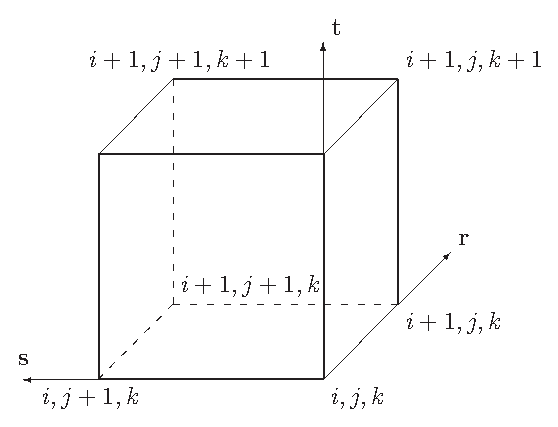
\includegraphics{cnct.figs/cnct_struct}
\end{minipage}%
\begin{minipage}[t]{0.45\linewidth}
   \vspace{-\abovedisplayskip}
   \begin{eqnarray*}
      W_{i,  j,  k  } &=& (1-r)(1-s)(1-t) \\
      W_{i+1,j,  k  } &=& r(1-s)(1-t) \\
      W_{i,  j+1,k  } &=& (1-r)s(1-t) \\
      W_{i,  j,  k+1} &=& (1-r)(1-s)t \\
      W_{i+1,j+1,k  } &=& rs(1-t) \\
      W_{i+1,j,  k+1} &=& r(1-s)t \\
      W_{i,  j+1,k+1} &=& (1-r)st \\
      W_{i+1,j+1,k+1} &=& rst
   \end{eqnarray*}
\end{minipage}}
\vspace{\baselineskip}

For unstructured grids, \texttt{InterpolantsDonor} is defined only for
the basic linear element types:
\texttt{BAR\_2}, \texttt{TRI\_3}, \texttt{QUAD\_4}, \texttt{TETRA\_4},
\texttt{PYRA\_5}, \texttt{PENTA\_6}, and \texttt{HEXA\_8}, defined in
\autoref{s:unstructgrid}.
The directionality for the $r$, $s$, and $t$ interpolants for the basic
element types is defined as follows.

\vspace{\baselineskip}
\texttt{BAR\_2}\\[-2\baselineskip]
\begin{center}
\begin{minipage}[t]{0.5\linewidth}
   \centering
   \vspace{0pt}
   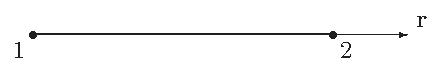
\includegraphics{cnct.figs/cnct_unst_bar2}
\end{minipage}%
\begin{minipage}[t]{0.5\linewidth}
   \vspace{-\abovedisplayskip}
   \begin{eqnarray*}
      W_1 &=& 1-r \\
      W_2 &=& r
   \end{eqnarray*}
\end{minipage}
\end{center}

\newpage
%\vspace{\baselineskip}
\texttt{TRI\_3}\\[-2\baselineskip]
\begin{center}
\begin{minipage}[t]{0.5\linewidth}
   \centering
   \vspace{0pt}
   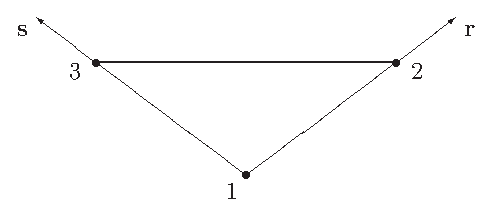
\includegraphics{cnct.figs/cnct_unst_tri3}
\end{minipage}%
\begin{minipage}[t]{0.5\linewidth}
   \vspace{-\abovedisplayskip}
   \begin{eqnarray*}
      W_1 &=& 1-r-s \\
      W_2 &=& r \\
      W_3 &=& s
   \end{eqnarray*}
\end{minipage}
\end{center}

\vspace{\baselineskip}
\texttt{QUAD\_4}\\[-2\baselineskip]
\begin{center}
\begin{minipage}[t]{0.5\linewidth}
   \centering
   \vspace{0pt}
   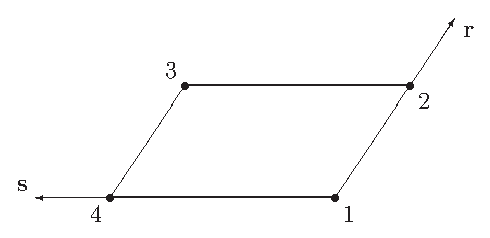
\includegraphics{cnct.figs/cnct_unst_quad4}
\end{minipage}%
\begin{minipage}[t]{0.5\linewidth}
   \vspace{-\abovedisplayskip}
   \begin{eqnarray*}
      W_1 &=& (1-r)(1-s) \\
      W_2 &=& r(1-s) \\
      W_3 &=& rs \\
      W_4 &=& (1-r)s
   \end{eqnarray*}
\end{minipage}
\end{center}

\vspace{\baselineskip}
\texttt{TETRA\_4}\\[-2\baselineskip]
\begin{center}
\begin{minipage}[t]{0.5\linewidth}
   \centering
   \vspace{0pt}
   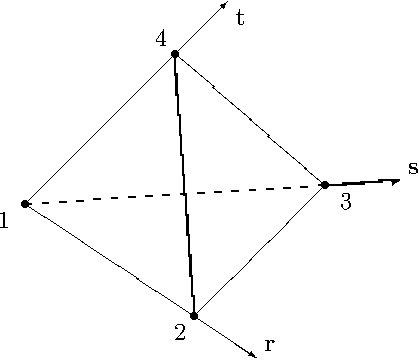
\includegraphics{cnct.figs/cnct_unst_tetra4}
\end{minipage}%
\begin{minipage}[t]{0.5\linewidth}
   \vspace{-\abovedisplayskip}
   \begin{eqnarray*}
      W_1 &=& 1-r-s-t \\
      W_2 &=& r \\
      W_3 &=& s \\
      W_4 &=& t
   \end{eqnarray*}
\end{minipage}
\end{center}

\newpage
%\vspace{\baselineskip}
\texttt{PYRA\_5}\\[-2\baselineskip]
\begin{center}
\begin{minipage}[t]{0.5\linewidth}
   \centering
   \vspace{0pt}
   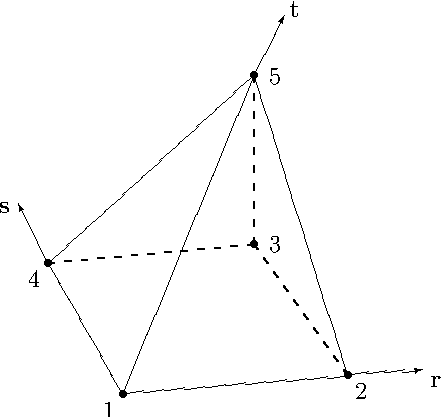
\includegraphics{cnct.figs/cnct_unst_pyra5}
\end{minipage}%
\begin{minipage}[t]{0.5\linewidth}
   \vspace{-\abovedisplayskip}
   \begin{eqnarray*}
      W_1 &=& (1-r)(1-s)(1-t) \\
      W_2 &=& r(1-s)(1-t) \\
      W_3 &=& rs(1-t) \\
      W_4 &=& (1-r)s(1-t) \\
      W_5 &=& t
   \end{eqnarray*}
\end{minipage}
\end{center}

\vspace{\baselineskip}
\texttt{PENTA\_6}\\[-2\baselineskip]
\begin{center}
\begin{minipage}[t]{0.5\linewidth}
   \centering
   \vspace{0pt}
   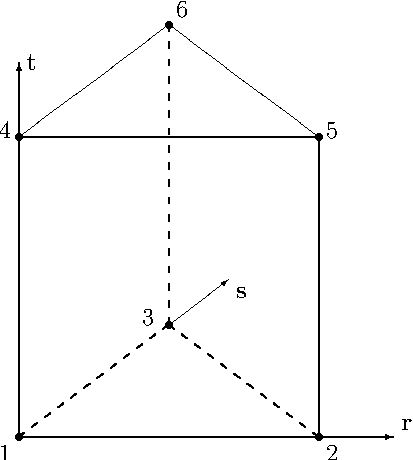
\includegraphics{cnct.figs/cnct_unst_penta6}
\end{minipage}%
\begin{minipage}[t]{0.5\linewidth}
   \vspace{-\abovedisplayskip}
   \begin{eqnarray*}
      W_1 &=& (1-r-s)(1-t) \\
      W_2 &=& r(1-t) \\
      W_3 &=& s(1-t) \\
      W_4 &=& (1-r-s)t \\
      W_5 &=& rt \\
      W_6 &=& st
   \end{eqnarray*}
\end{minipage}
\end{center}

\newpage
%\vspace{\baselineskip}
\texttt{HEXA\_8}\\[-2\baselineskip]
\begin{center}
\begin{minipage}[t]{0.5\linewidth}
   \centering
   \vspace{0pt}
   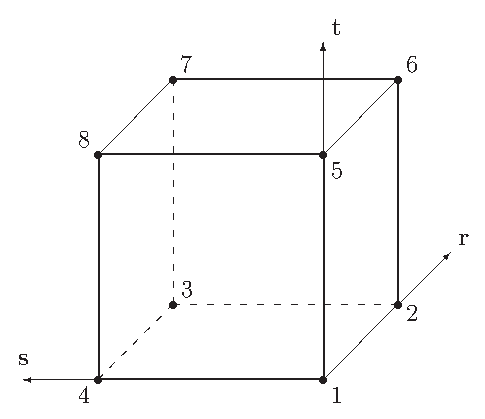
\includegraphics{cnct.figs/cnct_unst_hexa8}
\end{minipage}%
\begin{minipage}[t]{0.5\linewidth}
   \vspace{-\abovedisplayskip}
   \begin{eqnarray*}
      W_1 &=& (1-r)(1-s)(1-t) \\
      W_2 &=& r(1-s)(1-t) \\
      W_3 &=& rs(1-t) \\
      W_4 &=& (1-r)s(1-t) \\
      W_5 &=& (1-r)(1-s)t \\
      W_6 &=& r(1-s)t \\
      W_7 &=& rst \\
      W_8 &=& (1-r)st
   \end{eqnarray*}
\end{minipage}
\end{center}

\fort{PointListDonor} may only be used when the interface is
\fort{Abutting1to1}.
It contains the images of all the receiver-zone interface points in the
donor zone.
If the zone is structured, all indices in \fort{PointListDonor}
should have one index element in common.

For mismatched or overset interfaces, the zone connectivity
donor information, when given, is defined using either the
\fort{CellListDonor} alone, or the combination of \texttt{CellListDonor}
and \texttt{InterpolantsDonor}.
\fort{CellListDonor} contains the list of donor cells or elements in
which each node of the receiver zone can be located.
\fort{InterpolantsDonor} contains the interpolation factors to locate
the receiver nodes in the donor cells.
\fort{InterpolantsDonor} may be thought of as bi- or tri-linear
interpolants (depending on \fort{CellDimension}) in the cell of the
donor zone.

A \fort{GridConnectivityProperty\_t} data structure, described in
\autoref{s:GridConnectivityProperty}, may be used to record special
properties associated with particular connectivity patches, such as a
periodic interface, or an interface where data is to be averaged in some
way.

The \fort{UserDefinedData\_t} data structure allows arbitrary
user-defined data to be stored in \fort{Descriptor\_t} and
\fort{DataArray\_t} children without the restrictions or implicit
meanings imposed on these node types at other node locations.

|Ordinal| is user-defined and has no restrictions on the values that it can
contain.  It is included for backward compatibility to assist implementation
of the CGNS system into applications whose I/O depends heavily on the
numbering of zone interfaces.  Since there are no restrictions on the values
contained in |Ordinal| (or that |Ordinal| is even provided), there is no
guarantee that the interfaces for a given zone in an existing CGNS database
will have sequential values from 1 to $N$ without holes or repetitions.  Use
of |Ordinal| is discouraged and is on a user-beware basis.

\subsubsection*{FUNCTION \texttt{PointListSize}:}

\noindent return value: |int| \\
\noindent dependencies: |PointRange|, |PointList|

\fort{PointListDonor}, \fort{CellListDonor}, and \fort{InterpolantsDonor}
require the function \fort{PointListSize}, to identify the length of the
array.
If \fort{PointRange} is specified by \fort{GridConnectivity\_t},
then \fort{PointListSize} is obtained from the number of grid points
(inclusive) between the beginning and ending indices of \fort{PointRange}.
If \fort{PointList} is specified by \fort{GridConnectivity\_t},
then \fort{PointListSize} is actually a user input during creation of
the database; it is the length of the array \fort{PointList} whose
elements are also user inputs (by ``user'' we mean the application code
that is generating the CGNS database).

By definition, the |PointList| and |PointListDonor| arrays have the
same size, and this size should be stored along with the arrays in
their respective |IndexArray_t| structures.
|PointListSize| was chosen to be a structure function, rather than a
separate element of |GridConnectivity_t| for the following reasons:
first, it is redundant if |PointRange| is specified; and second, it
leads to redundant storage if |PointList| is specified, since the value
of |PointListSize| is also stored within the |PointList| structure.

This situation has somewhat of a precedent within the SIDS definitions.
The structure \fort{Descriptor\_t} contains a string of unspecified length.
Yet in  actual implementation, the (string) length is a function of the
descriptor string itself and should be stored along with the string.

\subsection{General Interface Connectivity Examples}
\label{s:cnct_gen_example}

\begin{example}{Structured Abutting Zones}
\label{ex:struct_abut}

Say that you have a three-dimensional structured grid.
Assume that at the interface between two zones you have the 
situation shown in \autoref{f:cnct_example1}.

\begin{figure}[!htb]
   \centering
   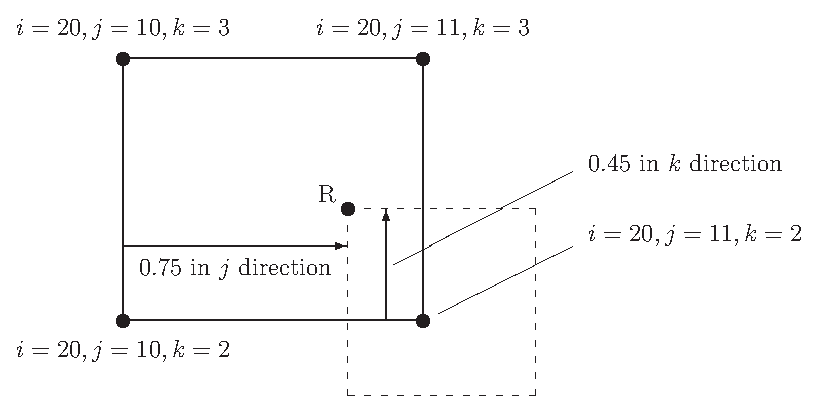
\includegraphics{cnct.figs/cnct_example1}
   \caption{Example Interface for Generalized Connectivity, Structured Grids}
   \label{f:cnct_example1}
\end{figure}

In this particular example, the patching occurs on a ``plane''.
In other words, the two cells in 3-D have faces that abut in a 2-D
sense.
It is these faces that we are picturing here.
The solid quadrilateral is the donor cell face, and the dashed
quadrilateral is the position of the receiving cell face relative to the
donor cell.
Note that since this is a 2-D-type of abutting case, one of the indices
(in this case $i = 20$, which represents \texttt{imax}) of the
donor cell is constant.
For this example, the point R of the receiver cell is located within the
donor cell pictured, and we wish to give the \texttt{CellListDonor} and
\texttt{InterpolantsDonor} for it.

Because this is a structured grid, the \texttt{CellListDonor} in this
case is given by
\begin{alltt}
   CellListDonor = (19, 10, 2)
\end{alltt}

Here, we are using the ``Structured Grid Notation and Indexing
Conventions'' (see \autoref{s:structgrid}) that say cell centers, face
centers, and edge centers are indexed by the minimum $i$, $j$, and $k$
indices of the connecting vertices.

The \texttt{InterpolantsDonor} defines an interpolation value relative
to the cell/element vertices.
In this case, say that the point R is located 0.75 along the
$j$-index direction and 0.45 along the $k$-index direction.
(It also lies on the $i = 20$, or \texttt{imax} face.)
Thus, in this example:
\begin{alltt}
   InterpolantsDonor = (1.0, 0.75, 0.45) 
\end{alltt}
Note that if the donor zone was instead located on an $i = 1$
(\texttt{imin} face), then the \texttt{CellListDonor} would be (1, 10, 2)
and the \texttt{InterpolantsDonor} would be (0.0, 0.75, 0.45).
\end{example}

\begin{example}{Unstructured Abutting Zones, \texttt{HEXA\_8} Donor Cell}
\label{ex:unstruct_abut1}

As a second example, assume that you have the same setup as before, but
now with a three-dimensional unstructured grid, shown in
\autoref{f:cnct_example2}.
In this case, we no longer have a 3-D array of indices defining
coordinate directions.
Instead, we simply have a 1-D list of indices as well as a list of
volume (and possibly face) elements composed of those indices.
In this example we again are assuming the two zones abut in a 2-D sense.
We now have the choice of describing the donor in terms of its volume
element or its boundary (face) element, if available.
Here in this example, we use the volume element.

\begin{figure}[!htb]
   \centering
   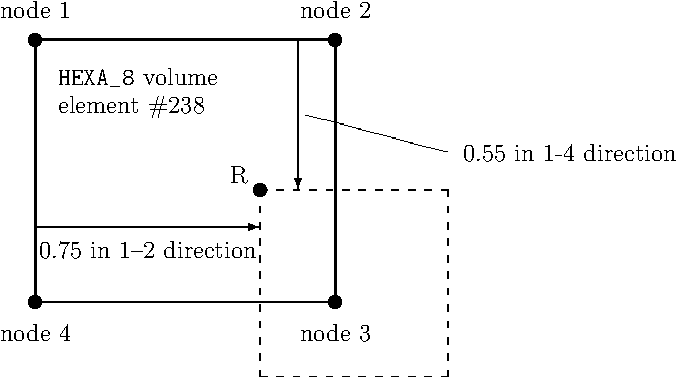
\includegraphics{cnct.figs/cnct_example2}
   \caption{Example Interface for Generalized Connectivity, Unstructured
            Grids with \texttt{HEXA\_8} Donor Cell}
   \label{f:cnct_example2}
\end{figure}

The \texttt{HEXA\_8} volume element has been appropriately numbered,
using the ``Unstructured Grid Element Numbering Conventions'' defined in
\autoref{s:unstructgrid}.
In this example, it is the 1-2-3-4 face of the volumetric element that
is abutting with the other zone (but it could be any of its six faces)

The \texttt{CellListDonor} in this case is simply given by
\begin{alltt}
   CellListDonor = (238)
\end{alltt}
Using the convention established above for \texttt{HEXA\_8} elements, the
\texttt{InterpolantsDonor} would be
\begin{alltt}
   InterpolantsDonor = (0.75, 0.55, 0.0)
\end{alltt}
\end{example}

\begin{example}{Unstructured Abutting Zones, \texttt{TRI\_3} Donor Cell}
\label{ex:unstruct_abut2}

As a third example, assume that you have two zones in a
three-dimensional unstructured grid with triangles and quadrilaterals at
its boundaries, as shown in \autoref{f:cnct_example3}.
Here the current zone (made up of quadrilateral faces) is abutting the
donor zone (made up of triangular faces) in a 2-D sense.
We again have the choice of describing the donor in terms of its volume
element or its boundary (face) element.
Here in this example, we use the face element.

\begin{figure}[!htb]
   \centering
   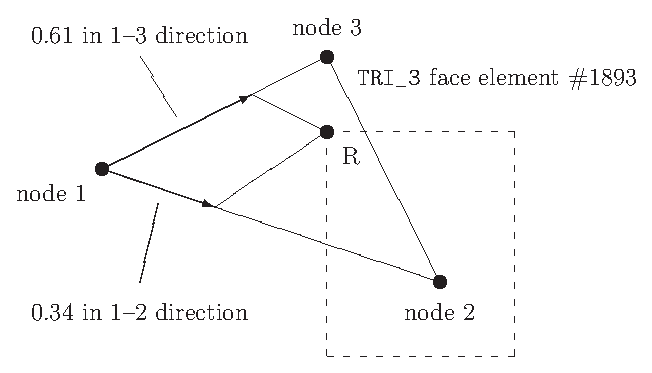
\includegraphics{cnct.figs/cnct_example3}
   \caption{Example Interface for Generalized Connectivity, Unstructured
            Grids with \texttt{TRI\_3} Donor Cell}
   \label{f:cnct_example3}
\end{figure}

The \texttt{CellListDonor} in this case is simply given by
\begin{alltt}
   CellListDonor = (1893)
\end{alltt}
Using the convention established above for \texttt{TRI\_3} elements, the
\texttt{InterpolantsDonor} would be:
\begin{alltt}
   InterpolantsDonor = (0.34, 0.61)
\end{alltt}
In this case the third dimension of the \texttt{InterpolantsDonor}
(although present) is not used, because by default the interpolation is
only two-dimensional in the 2-D plane of the donor face.
\end{example}

\subsection{Grid Connectivity Property Structure Definition: \texttt{GridConnectivityProperty\_t}}
\label{s:GridConnectivityProperty}

\fort{GridConnectivityProperty\_t} allows the recording of special
properties associated with particular connectivity patches.
At the current time, only two properties (\fort{Periodic\_t} and
\fort{AverageInterface\_t}) are included, but extensions involving
other properties may be implemented as additional nodes under
\fort{GridConnectivityProperty\_t} in the future.

\begin{alltt}
  GridConnectivityProperty\_t :=
    \{
    List( Descriptor\_t Descriptor1 ... DescriptorN ) ;                      (o)

    Periodic\_t Periodic ;                                                   (o)

    AverageInterface\_t AverageInterface ;                                   (o)

    List( UserDefinedData\_t UserDefinedData1 ... UserDefinedDataN ) ;       (o)
    \} ;
\end{alltt}

\begin{notes}
\item
 Default names for the \fort{Descriptor\_t} and
 \fort{UserDefinedData\_t}
 lists are as shown; users may choose other legitimate names.
 Legitimate names must be unique within a given instance of
 \fort{GridConnectivityProperty\_t} and shall not include the names
 \fort{Periodic} or \fort{AverageInterface}.
\end{notes}

The \fort{Periodic\_t} and \fort{AverageInterface\_t} data structures
may be used to record properties associated with periodic interfaces, or
interfaces where data is to be averaged in some way, respectively.

The \fort{UserDefinedData\_t} data structure allows arbitrary
user-defined data to be stored in \fort{Descriptor\_t} and
\fort{DataArray\_t} children without the restrictions or implicit
meanings imposed on these node types at other node locations.

\subsubsection{Periodic Interface Structure Definition: \texttt{Periodic\_t}}
\label{s:Periodic}

The \fort{Periodic\_t} data structure allows data associated with
a periodic interface to be recorded.

\begin{alltt}
  Periodic\_t :=
    \{
    List( Descriptor\_t Descriptor1 ... DescriptorN ) ;                      (o)

    DataArray\_t<real, 1, PhysicalDimension> RotationCenter ;                (r)
    DataArray\_t<real, 1, PhysicalDimension> RotationAngle ;                 (r)
    DataArray\_t<real, 1, PhysicalDimension> Translation ;                   (r)

    DataClass\_t DataClass ;                                                 (o)

    DimensionalUnits\_t DimensionalUnits ;                                   (o)

    List( UserDefinedData\_t UserDefinedData1 ... UserDefinedDataN ) ;       (o)
    \} ;
\end{alltt}

\begin{notes}
\item
 Default names for the \fort{Descriptor\_t} and
 \fort{UserDefinedData\_t} lists are as shown; users may choose other
 legitimate names.
 Legitimate names must be unique within a given instance of
 \fort{Periodic\_t} and shall not include the names \fort{DataClass},
 \fort{DimensionalUnits}, \fort{RotationAngle}, \fort{RotationCenter},
 or \fort{Translation}.
\end{notes}

\fort{RotationCenter} is the origin for defining the rotation angle
between the periodic interfaces.
\fort{RotationAngle} defines the angle from the current interface to
the connecting interface.
If rotating about more than one axis, the rotation is performed first
about the x-axis, then the y-axis, then the z-axis.
\fort{Translation} defines the translation from the current interface
to the connecting interface.

\fort{DataClass} defines the default for the class of data contained in
the \fort{DataArray\_t} structures.
If the data is dimensional, \fort{DimensionalUnits} may be used to
describe the system of dimensional units employed.
If present, these two entities take precedence of all corresponding
entities at higher levels of the hierarchy.
These precedence rules are further discussed in \autoref{s:precedence}.

The \fort{UserDefinedData\_t} data structure allows arbitrary
user-defined data to be stored in \fort{Descriptor\_t} and
\fort{DataArray\_t} children without the restrictions or implicit
meanings imposed on these node types at other node locations.

\subsubsection{Average Interface Structure Definition: \texttt{AverageInterface\_t}}
\label{s:AverageInterface}

The \fort{AverageInterface\_t} data structure is used when data at the
current connectivity interface is to be averaged in some way prior to
passing it to a neighboring interface.

\begin{alltt}
  AverageInterface\_t :=
    \{
    List( Descriptor\_t Descriptor1 ... DescriptorN ) ;                      (o)

    AverageInterfaceType\_t AverageInterfaceType ;                           (r)

    List( UserDefinedData\_t UserDefinedData1 ... UserDefinedDataN ) ;       (o)
    \} ;
\end{alltt}

\begin{notes}
\item
 Default names for the \fort{Descriptor\_t} and
 \fort{UserDefinedData\_t} lists are as shown; users may choose other
 legitimate names.
 Legitimate names must be unique within a given instance of
 \fort{AverageInterface\_t} and shall not include the name
 \fort{AverageInterfaceType}.
\end{notes}

\fort{AverageInterfaceType\_t} is a required enumeration data structure
that is used to define the type of averaging to be done.
\begin{alltt}
  AverageInterfaceType_t := Enumeration(
    AverageInterfaceTypeNull,
    AverageInterfaceTypeUserDefined,
    AverageAll,
    AverageCircumferential,
    AverageRadial,
    AverageI,
    AverageJ,
    AverageK ) ;
\end{alltt}

\fort{AverageAll} means that the data from the entire current patch is
averaged, whereas each of the other choices indicates averaging of the
data on the current interface in the indicated direction.
Note that \fort{AverageI}, \fort{AverageJ}, and \fort{AverageK}
apply only to structured grids.

The \fort{UserDefinedData\_t} data structure allows arbitrary
user-defined data to be stored in \fort{Descriptor\_t} and
\fort{DataArray\_t} children without the restrictions or implicit
meanings imposed on these node types at other node locations.

\subsection{Overset Grid Holes Structure Definition: \texttt{OversetHoles\_t}}
\label{s:OversetHoles}

Grid connectivity for overset grids must also include ``holes'' within zones,
where any solution states are ignored or ``turned off'', because they are
solved for in some other overlapping zone.  The structure |OversetHoles_t|
specifies those points within a given zone that make up a hole (or holes),
and applies to both structured and unstructured zones.
Grid points specified in this structure are equivalent to those with
IBLANK=0 in the PLOT3D format.

\begin{alltt}
  OversetHoles\_t< int IndexDimension > :=
    \{
    List( Descriptor\_t Descriptor1 ... DescriptorN ) ;                      (o)

    GridLocation\_t GridLocation ;                                           (o/d)

    List( IndexRange\_t<IndexDimension> 
      PointRange, PointRange2 ... PointRangeN ) ;                           (o:r)

    IndexArray\_t<IndexDimension, PointListSize, int> PointList ;            (r:o)

    List( UserDefinedData\_t UserDefinedData1 ... UserDefinedDataN ) ;       (o)
    \} ;
\end{alltt}

\begin{notes}
\item
 Default names for the \fort{Descriptor\_t}, \fort{IndexRange\_t}, and
 \fort{UserDefinedData\_t}
 lists are as shown; users may choose other legitimate names.
 Legitimate names must be unique 
 within a given instance of \fort{OversetHoles\_t} and shall not include the
 names \fort{GridLocation} or \fort{PointList}.
\item
 If |GridLocation| is absent, then its default value is |Vertex|.
\item
 One of |PointRange| and |PointList| must be specified, but not both.
\end{notes}

The location of grid indices specified in \fort{PointList} and the
\fort{PointRange} list is given by \fort{GridLocation}.

The grid points making up a hole within a zone may be specified by
|PointRange| if they constitute a logically rectangular region.  If the hole
points constitute a (small) set of possibly overlapping logically rectangular
regions, then they may be specified by the list |PointRange|, |PointRange2|,
etc.  The more general alternate is to use |PointList| to list all grid
points making up the hole(s) within a zone.
Note that using multiple |PointRange| specifications may result in a
given hole being specified more than once.

The \fort{UserDefinedData\_t} data structure allows arbitrary
user-defined data to be stored in \fort{Descriptor\_t} and
\fort{DataArray\_t} children without the restrictions or implicit
meanings imposed on these node types at other node locations.

\subsubsection*{FUNCTION \texttt{PointListSize}:}

\noindent return value: |int| \\
\noindent dependencies: |PointList|

|OversetHoles_t| requires one structure function, |PointListSize|, to 
identify the length of the |PointList| array.
|PointListSize| is a user input.
(See the discussion on function |PointListSize| in
\autoref{s:GridConnectivity}).
